\documentclass[11pt,a4paper]{article}
\usepackage[utf8]{inputenc}
\usepackage[T1]{fontenc}
\usepackage{geometry}
\usepackage{hyperref}
\usepackage{enumitem}
\usepackage{booktabs}
\usepackage{array}
\usepackage{float}
\usepackage{xcolor}
\usepackage{colortbl}
\usepackage{graphicx}
\usepackage{tikz}
\usetikzlibrary{positioning}
\usepackage{eso-pic}
\usepackage[most]{tcolorbox}
\usepackage{pifont}
\usepackage{fontawesome5}
\usepackage{titlesec}
\usepackage{tabularx}

% Remove link borders; use black link colors
\hypersetup{
  colorlinks=true,
  linkcolor=black,
  urlcolor=black,
  citecolor=black,
  pdfborder={0 0 0}
}

% Brand color
\definecolor{linqraprimary}{HTML}{ED7534}
\definecolor{linqrablue}{RGB}{0,102,204}

% Paragraph spacing: one line gap; remove indent
% Keep headings tight to the following paragraph
\setlength{\parskip}{1\baselineskip}
\setlength{\parindent}{0pt}
\titlespacing*{\section}{0pt}{*2}{0pt}
\titlespacing*{\subsection}{0pt}{*1.5}{0pt}
\titlespacing*{\subsubsection}{0pt}{*1.2}{0pt}

% Left vertical brand bar on every page
\AddToShipoutPictureBG{%
  \begin{tikzpicture}[remember picture,overlay]
    \fill[linqraprimary] (current page.north west) ++(0,-0.75cm) rectangle ++(0.25cm,-\paperheight+1.5cm);
  \end{tikzpicture}%
}
\usepackage{tikz}
\usetikzlibrary{positioning,calc}

% Remove red link borders and use clean black links
\hypersetup{
  colorlinks=true,
  linkcolor=black,
  urlcolor=black,
  citecolor=black,
  pdfborder={0 0 0}
}

\geometry{margin=1in}

\title{\textbf{Linqra: Unifying AI Integrations for the Modern Enterprise}}\author{Mehmet Timur Sen \\ Fatih David Sen}\date{\today}

\begin{document}

% Title block with logo
\begin{center}
\vspace*{2.5cm}

\includegraphics[width=0.55\textwidth]{linqra_logo}
\vspace{1.8cm}

{\Huge \textbf{Linqra: Unifying AI Integrations for the Modern Enterprise}}\\[16pt]
\vspace{1.8cm}
{\LARGE Mehmet Timur Sen}\\[6pt]
\vspace{0.2cm}
{\LARGE Fatih David Sen}\\[12pt]
{\large \today}
\end{center}

\vfill

\begin{center}
\textbf{Website:} \href{https://linqra.com}{linqra.com}
\end{center}

\newpage
\tableofcontents
\newpage

\newpage
\section{Executive Summary}
The rapid proliferation of Artificial Intelligence (AI) models from providers like OpenAI, Anthropic, Google, and Meta has created a paradigm of ``model sprawl'' for enterprises. While this diversity offers unprecedented potential, it introduces severe operational complexity. Development teams are burdened with managing multiple API integrations, each with unique authentication methods, rate limits, pricing models, and output formats. This fragmentation stifles innovation, creates security vulnerabilities, and leads to significant inefficiencies and hidden costs.

Linqra presents a definitive solution: a unified API gateway and orchestration platform designed to simplify multi-model AI integration. By standardizing access to a vast ecosystem of AI models through a single, secure endpoint, Linqra abstracts away the underlying complexity. The platform empowers developers to build, manage, and scale sophisticated AI agents and workflows with unparalleled speed, resilience, and cost-effectiveness.

This white paper details the challenges of the current multi-model landscape, outlines Linqra's technical architecture and the Linq Protocol, and demonstrates the tangible return on investment (ROI) for enterprises adopting a unified AI integration strategy.

\subsection*{Key Takeaways}
\begin{itemize}[leftmargin=1.8em]
  \item[\textcolor{linqraprimary}{\faIcon{tachometer-alt}}] \textbf{Eliminate Integration Overhead}: Reduce development time by up to 70\% by using a single, standardized API.
  \item[\textcolor{linqraprimary}{\faLifeRing}] \textbf{Enhance Resilience \& Performance}: Intelligently route requests to avoid downtime and leverage fallback models.
  \item[\textcolor{linqraprimary}{\faChartLine}] \textbf{Gain Granular Control \& Insights}: Monitor usage, manage costs, and optimize AI spend across the entire organization.
  \item[\textcolor{linqraprimary}{\faLayerGroup}] \textbf{Future-Proof Your AI Stack}: Seamlessly integrate new AI models as they emerge without code changes.
\end{itemize}

\begin{center}
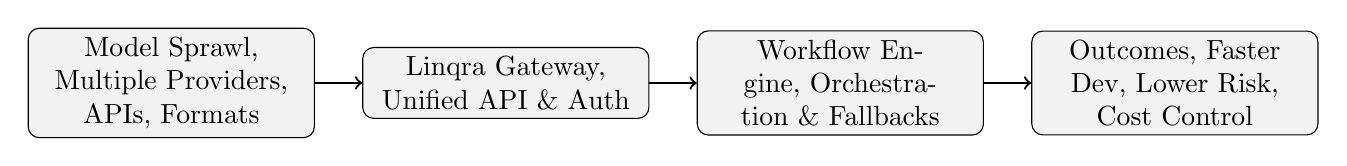
\begin{tikzpicture}[
  node distance=0.6cm,
  stage/.style={rectangle, draw, rounded corners, fill=gray!10, text width=3.4cm, align=center, anchor=center, minimum height=0.9cm},
  arrow/.style={->, thick}
]
\node[stage] (sprawl) {Model Sprawl, Multiple Providers, APIs, Formats};
\node[stage, right=of sprawl] (gateway) {Linqra Gateway, Unified API \& Auth};
\node[stage, right=of gateway] (engine) {Workflow Engine,  Orchestration \& Fallbacks};
\node[stage, right=of engine] (outcomes) {Outcomes, Faster Dev, Lower Risk, Cost Control};
\draw[arrow] (sprawl) -- (gateway);
\draw[arrow] (gateway) -- (engine);
\draw[arrow] (engine) -- (outcomes);
\end{tikzpicture}
\end{center}

\noindent\textbf{Call to Action:} Explore how Linqra can transform the AI development lifecycle. Visit \href{https://www.linqra.com}{linqra.com} to request a demo or start a free trial.

\newpage

\section{Introduction: The Age of AI Model Sprawl}
Enterprises are racing to leverage AI to gain a competitive edge, automate processes, and create innovative products. However, the AI landscape is no longer monolithic. The era of relying on a single large language model (LLM) is over. Today, development teams must strategically combine specialized models for coding, image generation, data analysis, and reasoning from a dozen different providers.

\begin{center}
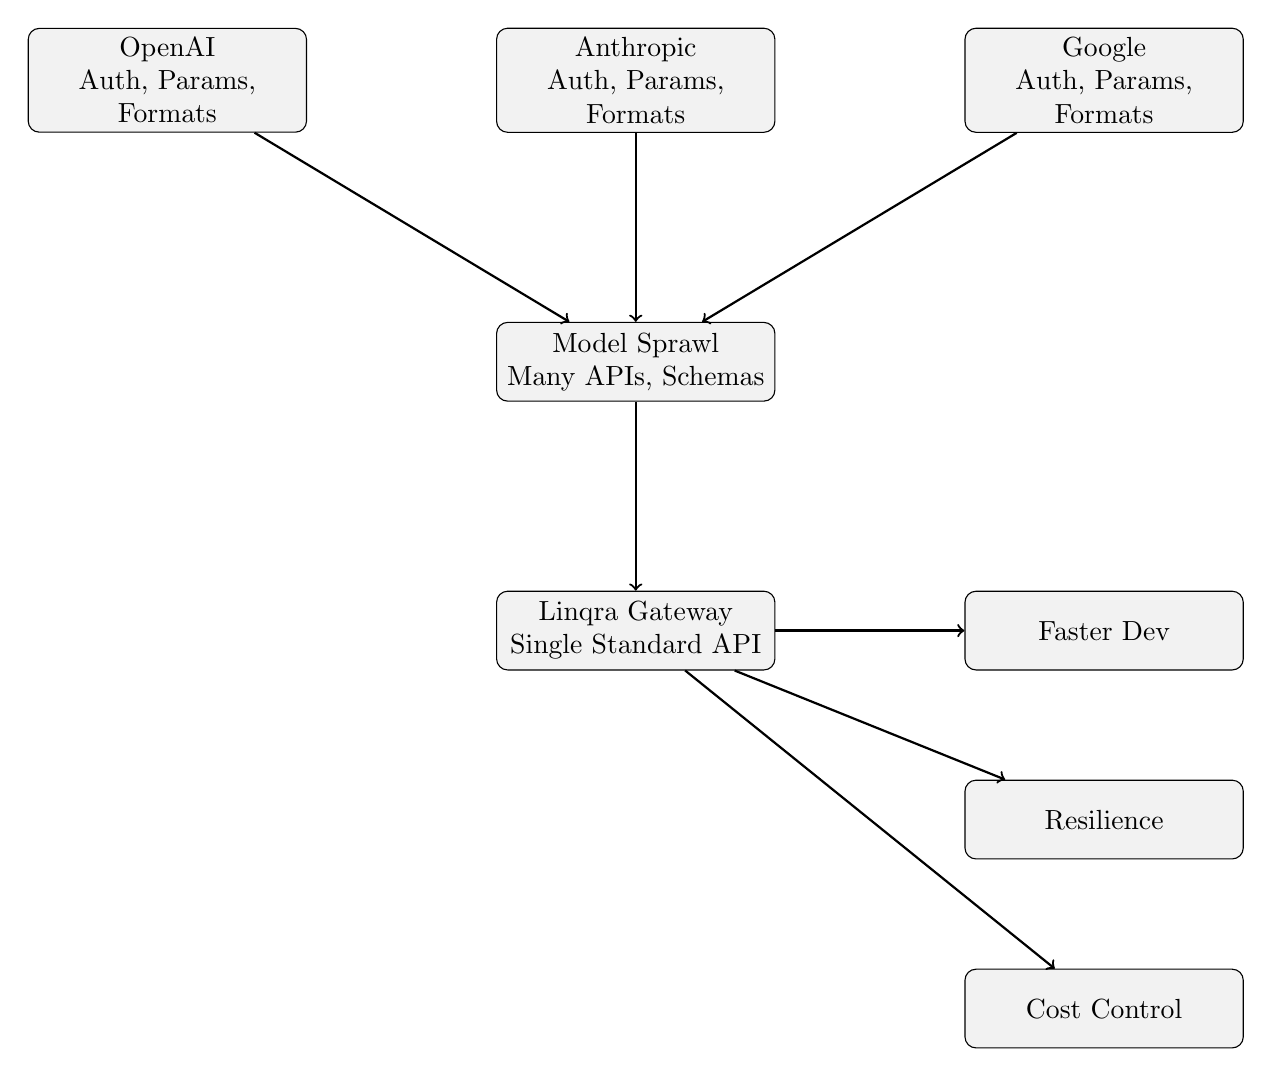
\begin{tikzpicture}[
  node distance=2.4cm,
  srv/.style={rectangle, draw, rounded corners, fill=gray!10, text width=3.3cm, align=center, minimum height=1cm},
  flow/.style={->, thick}
]
% Left: fragmented providers
\node[srv] (openai) {OpenAI\\Auth, Params, Formats};
\node[srv, right=of openai] (anthropic) {Anthropic\\Auth, Params, Formats};
\node[srv, right=of anthropic] (google) {Google\\Auth, Params, Formats};

% Middle: sprawl to gateway
\node[srv, below=of anthropic] (sprawl) {Model Sprawl\\Many APIs, Schemas};
\node[srv, below=of sprawl] (gateway) {Linqra Gateway\\Single Standard API};

% Right: outcomes
\node[srv, right=of gateway] (dev) {Faster Dev};
\node[srv, below of=dev] (res) {Resilience};
\node[srv, below of=res] (cost) {Cost Control};

\draw[flow] (openai) -- (sprawl);
\draw[flow] (anthropic) -- (sprawl);
\draw[flow] (google) -- (sprawl);
\draw[flow] (sprawl) -- (gateway);
\draw[flow] (gateway) -- (dev);
\draw[flow] (gateway) -- (res);
\draw[flow] (gateway) -- (cost);
\end{tikzpicture}
\end{center}

This diversity, while powerful, has created a new set of critical challenges. The ``build vs. integrate'' dilemma has never been more acute. Building custom integrations for each model is a time-consuming, error-prone, and maintenance-heavy task that distracts developers from core business logic. This paper addresses the pressing need for a centralized, intelligent layer to manage this complexity.

\newpage
\section{The Problem in Detail: The Hidden Costs of Multi-Model Integration}
The challenges of managing multiple AI integrations extend far beyond initial setup, creating ongoing friction and risk.

\begin{itemize}[leftmargin=1.8em]
  \item[\textcolor{linqraprimary}{\faCode}] \textbf{Development Inefficiency}: Engineers spend weeks, not hours, writing and maintaining boilerplate code for authentication, error handling, and data formatting for each API. This significantly slows time-to-market for AI-powered features.
  \item[\textcolor{linqraprimary}{\faRandom}] \textbf{Lack of Standardization}: Each provider has its own API schema, parameters, and response structures. Switching a feature from one model to another for cost or performance reasons often requires a complete code rewrite.
  \item[\textcolor{linqraprimary}{\faLock}] \textbf{Security and Compliance Risks}: Managing multiple API keys across different environments (development, staging, production) increases the attack surface. Ensuring consistent security policies and audit trails across all AI interactions becomes a compliance nightmare.
\end{itemize}

\newpage
\section{The Linqra Solution: A Unified Gateway for AI}
Linqra solves these challenges by acting as a universal adapter between applications and the entire ecosystem of AI models. The platform is built on two core concepts:

\begin{center}
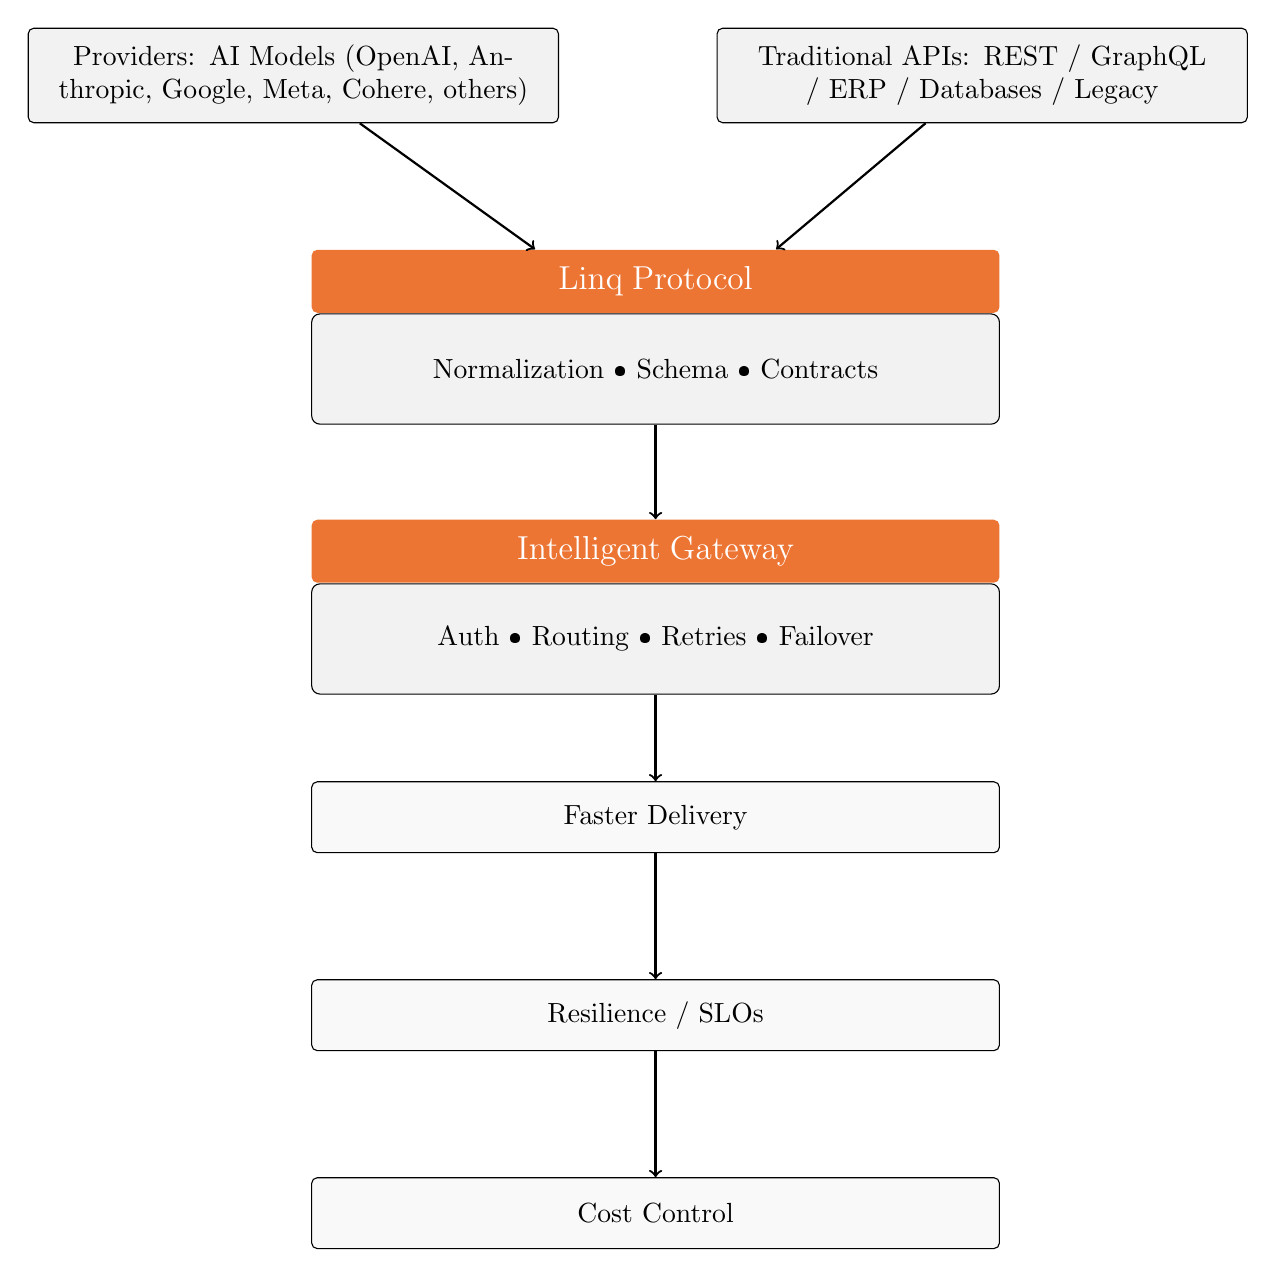
\begin{tikzpicture}[
  node distance=1.6cm,
  cluster/.style={rectangle, draw, rounded corners=2pt, fill=gray!10, text width=6.5cm, minimum height=1.2cm, align=center},
  header/.style={rectangle, rounded corners=2pt, fill=linqraprimary, text=white, text width=8.5cm, minimum height=0.8cm, align=center},
  block/.style={rectangle, draw, rounded corners=3pt, fill=gray!10, text width=8.5cm, minimum height=1.4cm, align=center},
  outcome/.style={rectangle, draw, rounded corners=2pt, fill=gray!5, text width=8.5cm, minimum height=0.9cm, align=center},
  arrow/.style={->, thick}
]
\node[cluster] (providers) {Providers: AI Models (OpenAI, Anthropic, Google, Meta, Cohere, others)};
\node[cluster, right=2.0cm of providers] (apis) {Traditional APIs: REST / GraphQL / ERP / Databases / Legacy};
\node[header, below=1.6cm of providers, xshift=4.6cm] (lp_h) {\large Linq Protocol};
\node[block, below=0cm of lp_h] (lp_b) {Normalization \textbullet{} Schema \textbullet{} Contracts};
\node[header, below=1.2cm of lp_b] (gw_h) {\large Intelligent Gateway};
\node[block, below=0cm of gw_h] (gw_b) {Auth \textbullet{} Routing \textbullet{} Retries \textbullet{} Failover};
\node[outcome, below=1.1cm of gw_b] (o1) {Faster Delivery};
\node[outcome, below=of o1] (o2) {Resilience / SLOs};
\node[outcome, below=of o2] (o3) {Cost Control};
\draw[arrow] (providers) -- ($(lp_h.north west)!0.65!(lp_h.north)$);
\draw[arrow] (apis) -- ($(lp_h.north east)!0.65!(lp_h.north)$);
\draw[arrow] (lp_b) -- (gw_h);
\draw[arrow] (gw_b) -- (o1);
\draw[arrow] (o1.south) -- (o2.north);
\draw[arrow] (o2.south) -- (o3.north);
\end{tikzpicture}
\end{center}

\subsection{The Linq Protocol}
A standardized, provider-agnostic API specification. Developers integrate once with the Linqra gateway and gain instant access to all supported models. The protocol normalizes requests and responses, allowing for seamless model interoperability.

\subsection{The Intelligent Gateway}
A high-performance routing layer that handles authentication, load balancing, retries, and failover intelligently. It translates a single request from the Linq Protocol into the specific format required by the target provider(s).

\newpage
\section{Technical Architecture: How Linqra Works}
The Linqra platform is engineered for scale, security, and flexibility. The architecture flows through a logical pipeline:

\begin{center}
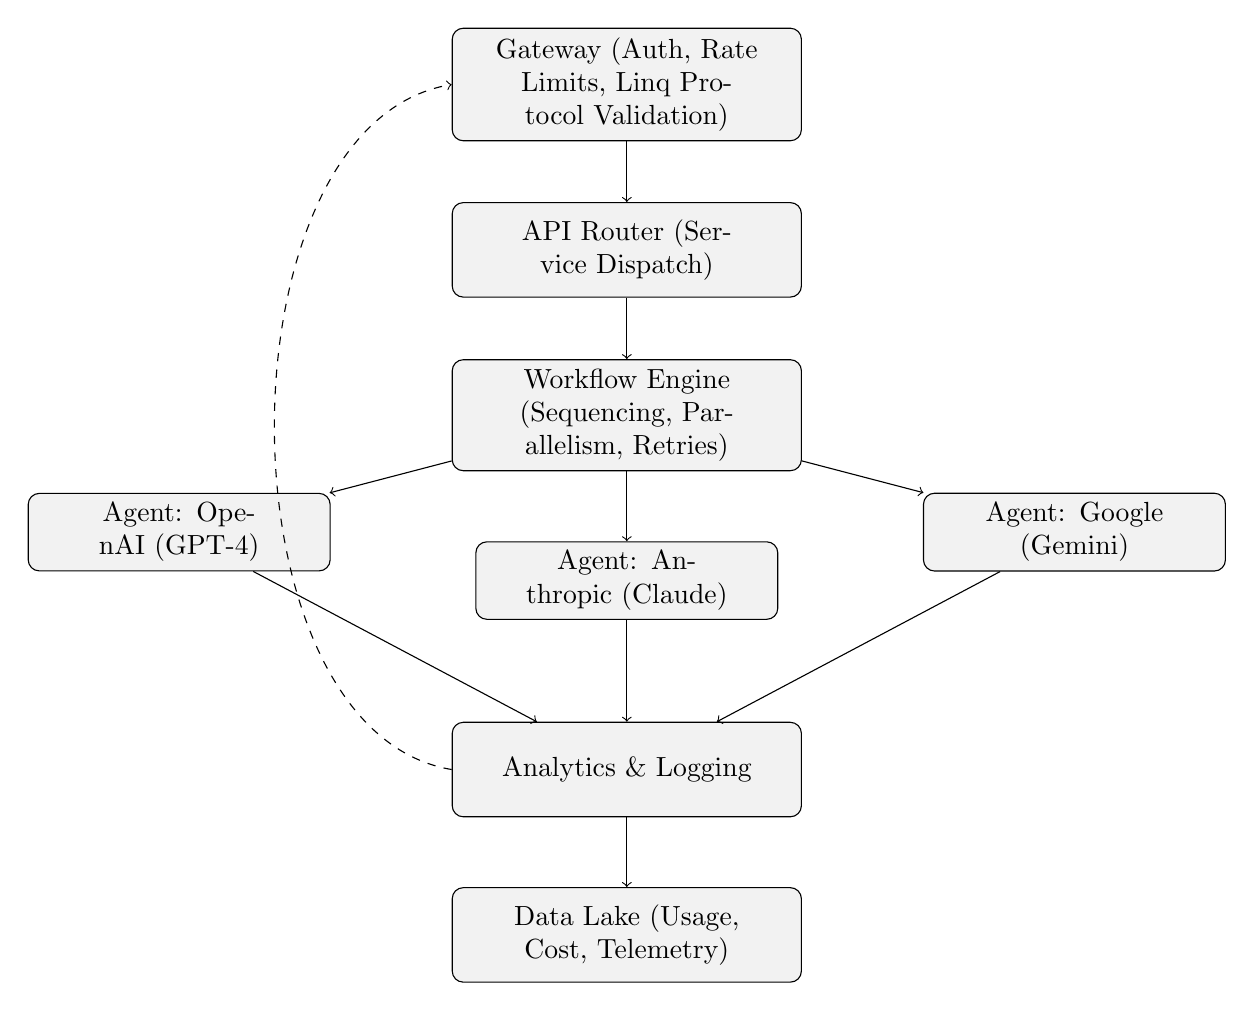
\begin{tikzpicture}[
  node distance=2.1cm,
  box/.style={rectangle, draw, rounded corners, fill=gray!10, text width=4.2cm, text centered, minimum height=1.2cm},
  small/.style={rectangle, draw, rounded corners, fill=gray!10, text width=3.6cm, text centered, minimum height=0.9cm}
]

% Top entry
\node[box] (gateway) {Gateway (Auth, Rate Limits, Linq Protocol Validation)};

% Router
\node[box, below of=gateway] (router) {API Router (Service Dispatch)};

% Workflow Engine
\node[box, below of=router] (engine) {Workflow Engine (Sequencing, Parallelism, Retries)};

% Agents row
\node[small, below left of=engine, xshift=-4.2cm] (agent1) {Agent: OpenAI (GPT-4)};
\node[small, below of=engine] (agent2) {Agent: Anthropic (Claude)};
\node[small, below right of=engine, xshift=4.2cm] (agent3) {Agent: Google (Gemini)};

% Analytics / Data Lake
\node[box, below of=agent2, yshift=-0.3cm] (analytics) {Analytics \& Logging};
\node[box, below of=analytics] (datalake) {Data Lake (Usage, Cost, Telemetry)};

% Arrows
\draw[->] (gateway) -- (router);
\draw[->] (router) -- (engine);
\draw[->] (engine) -- (agent1);
\draw[->] (engine) -- (agent2);
\draw[->] (engine) -- (agent3);
\draw[->] (agent1) -- (analytics);
\draw[->] (agent2) -- (analytics);
\draw[->] (agent3) -- (analytics);
\draw[->] (analytics) -- (datalake);

% Feedback loop (dashed)
\draw[->, dashed] (analytics.west) .. controls +(-3,0.5) and +(-3,-0.5) .. (gateway.west);

\end{tikzpicture}
\end{center}

\begin{itemize}[leftmargin=*]
  \item \textbf{Gateway}: The secure entry point. It authenticates the request, validates it against the Linq Protocol, and applies rate limiting and usage quotas.
  \item \textbf{API Router}: Directs the request to the appropriate internal service, whether a direct model call or a complex workflow.
  \item \textbf{Workflow Engine (Orchestration)}: For advanced use cases, this component allows the chaining of multiple AI agents in a defined sequence or in parallel. For example, an input could be first analyzed by a reasoning model, then sent to a coding model, with the result finally checked by a validation model.
  \item \textbf{Agents}: Configured connectors to specific AI providers (e.g., OpenAI GPT-4, Anthropic's Claude). They handle the final translation of the standardized request into the provider-specific API call.
  \item \textbf{Analytics \& Logging}: Every interaction is logged, analyzed, and fed into a data lake. This provides real-time insights into performance, cost, and usage patterns.
\end{itemize}

\newpage
\section{Key Features and Benefits}
\begin{table}[H]
\centering
\renewcommand{\arraystretch}{1.3}
\setlength{\tabcolsep}{8pt}
\begin{tabular}{p{0.30\textwidth} p{0.65\textwidth}}
\toprule
\textbf{Feature} & \textbf{Benefit to Your Enterprise} \\
\midrule
Single Standardized API & \textbf{Faster Development:} Drastically reduce integration time. Build and iterate on AI features faster than competitors. \\
Intelligent Routing \& Fallback & \textbf{Maximum Uptime:} Ensure application resilience. If a primary model is slow or down, Linqra automatically fails over to a backup model without dropping requests. \\
Unified Security \& Auth & \textbf{Reduced Risk:} Manage a single set of credentials. Enforce security policies consistently and simplify compliance reporting (SOC2, HIPAA, etc.). \\
Centralized Analytics \& Cost Management & \textbf{Optimized Spend:} Gain a holistic view of AI consumption. Identify cost-saving opportunities by comparing model performance for specific tasks. Set budgets and alerts to prevent overages. \\
Workflow Orchestration & \textbf{Leverage Best-of-Breed Models:} Easily build complex AI agents that leverage the unique strengths of different models within a single business process. \\
\bottomrule
\end{tabular}
\caption{Key Features and Enterprise Benefits}
\end{table}

\newpage
\section{Use Cases and Projected ROI}
\subsection{Use Case: Customer Support Automation}
An enterprise builds a support agent that uses a complex workflow:

\begin{enumerate}[leftmargin=*]
  \item \textbf{Step 1 (Agent A):} A large-context model (e.g., Claude) analyzes the customer's entire support history and current query.
  \item \textbf{Step 2 (Agent B):} A cost-effective model (e.g., GPT-3.5 Turbo) drafts a response based on the analysis.
  \item \textbf{Step 3 (Agent C):} A high-accuracy model (e.g., GPT-4) reviews and refines the draft for tone, accuracy, and compliance.
\end{enumerate}

Without Linqra, managing this three-step workflow across three different APIs would require significant custom code for sequencing, error handling, and data passing. With Linqra, it is configured declaratively via the workflow engine, reducing development time from weeks to days.

\subsection{Revenue Model and ROI}
Linqra operates on a transparent usage-based pricing model. The ROI is calculated from:

\begin{itemize}[leftmargin=1.8em]
  \item[\textcolor{linqraprimary}{\faCoins}] \textbf{Cost Savings:} Reduced developer hours spent on integration and maintenance.
  \item[\textcolor{linqraprimary}{\faIcon{shield-alt}}] \textbf{Risk Mitigation:} Value of avoiding downtime through resilient failover.
  \item[\textcolor{linqraprimary}{\faCogs}] \textbf{Operational Efficiency:} Savings from optimized model selection and preventing budget overruns.
  \item[\textcolor{linqraprimary}{\faRocket}] \textbf{Accelerated Innovation:} Revenue generated from getting AI products to market faster.
\end{itemize}

A typical enterprise customer realizes a full return on investment within 3--6 months through a combination of these factors.

\newpage

\section{Parallel Processing Architecture}

Linqra supports parallelized context gathering to minimize latency and improve downstream model quality. Independent retrieval tasks (product knowledge, customer history, similar cases, etc.) execute concurrently, and their outputs are merged into a unified context prior to orchestration. This reduces time-to-first-token and avoids serial bottlenecks.

\subsection{Context Gathering Parallelization}

\begin{figure}[H]
\centering
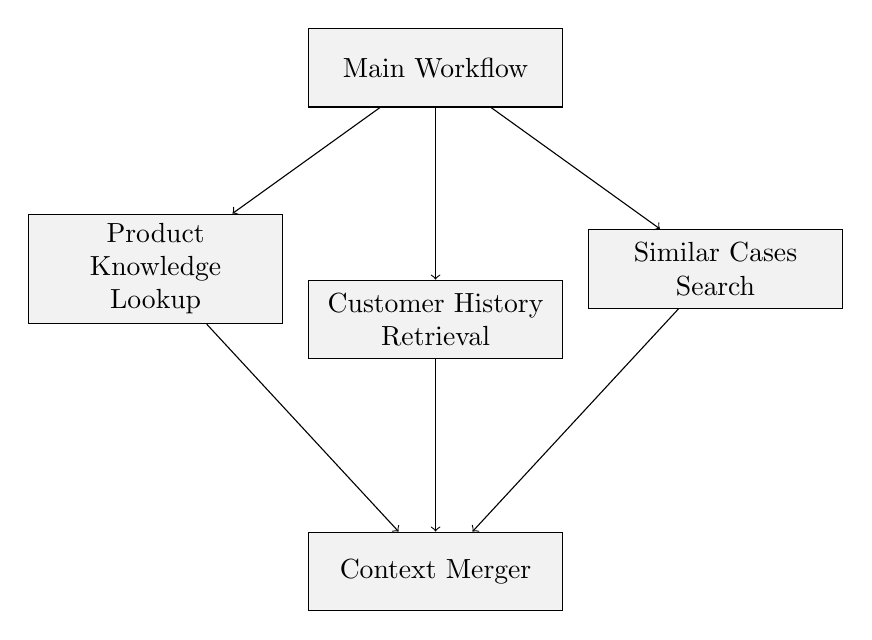
\begin{tikzpicture}[
    node distance=2.2cm,
    box/.style={rectangle, draw, fill=gray!10, text width=3cm, text centered, minimum height=1cm}
]

% Main workflow
\node[box] (main) {Main Workflow};

% Parallel context gathering
\node[box, below left of=main, xshift=-2cm, yshift=-1cm] (product) {Product Knowledge\\Lookup};
\node[box, below of=main, yshift=-1cm] (history) {Customer History\\Retrieval};
\node[box, below right of=main, xshift=2cm, yshift=-1cm] (cases) {Similar Cases\\Search};

% Merge point
\node[box, below of=history, yshift=-1cm] (merge) {Context Merger};

% Arrows
\draw[->] (main) -- (product);
\draw[->] (main) -- (history);
\draw[->] (main) -- (cases);
\draw[->] (product) -- (merge);
\draw[->] (history) -- (merge);
\draw[->] (cases) -- (merge);

\end{tikzpicture}
\caption{Parallel Context Gathering Architecture}
\end{figure}

\newpage
\section{Monitoring and Analytics}

Linqra provides comprehensive observability across the workflow lifecycle. Metrics are captured at request, step, and model tiers; they feed live dashboards and automated alerts to keep quality, reliability, and spend under control.

\subsection{Real-time Metrics}

\begin{itemize}
    \item \textbf{Execution Progress}: Step-by-step status across orchestration, including queue time, start/end timestamps, and per-step outcomes.
    \item \textbf{Confidence Scores}: Model- or validator-provided confidence signals used for quality gates and fallback routing.
    \item \textbf{Quality Gate Status}: Pass/fail with reasons for each configured gate; distributions to tune thresholds.
    \item \textbf{Resource Usage}: CPU, memory, tokens, and API call volume; used for capacity planning and rate-limit protection.
    \item \textbf{Error Rates}: Failure classes (timeouts, rate limits, provider errors) with retry effectiveness and MTTR.
\end{itemize}

\subsection{Performance Dashboards}

\begin{table}[H]
\centering
\renewcommand{\arraystretch}{1.25}
\setlength{\tabcolsep}{6pt}
\begin{tabularx}{\textwidth}{|l|l|X|}
\hline
\textbf{Dashboard} & \textbf{Metrics} & \textbf{Alert Thresholds} \\
\hline
Execution Time & Avg, P95, P99 & > 300s (Warn), > 600s (Crit) \\
Success Rate & Overall, by step & < 97\% (Warn), < 95\% (Crit) \\
Quality Scores & Avg, distribution & < 0.85 (Warn), < 0.80 (Crit) \\
Resource Usage & CPU, Mem, API calls & > 80\% (Warn), > 90\% (Crit) \\
\hline
\end{tabularx}
\caption{Monitoring Dashboard Configuration}
\end{table}

\small
\noindent\textit{Rationale:}
\begin{itemize}[leftmargin=*]
  \item \textbf{Execution Time}: High latency degrades UX; investigate upstream latency, provider slowness, or queue backlogs.
  \item \textbf{Success Rate}: Reliability issues and rising retries/cost; examine failing steps and providers.
  \item \textbf{Quality Scores}: Quality gates triggering; adjust prompts/models, validate inputs, or tune thresholds.
  \item \textbf{Resource Usage}: Capacity pressure; risk of throttling; scale workers or tune concurrency/rate limits.
\end{itemize}
\normalsize

\newpage
\section{Conclusion and Next Steps}
The complexity of multi-model AI integration is not a temporary hurdle; it is the new reality. Enterprises that attempt to manage this complexity with ad-hoc, point-to-point integrations will find themselves at a significant disadvantage, burdened by technical debt, security gaps, and spiraling costs.

Linqra provides the strategic foundation necessary to harness the full power of the modern AI ecosystem. By adopting a unified API gateway, organizations can shift focus from managing infrastructure to driving innovation.

\subsection*{Recommended Next Steps}
\begin{enumerate}[leftmargin=*]
  \item \textbf{Assess Your Integration Overhead:} Audit current AI integrations to quantify development and maintenance effort.
  \item \textbf{Identify a Pilot Project:} Select a non-critical but meaningful project that uses 2--3 different AI models.
  \item \textbf{Experience the Difference:} See Linqra in action.
\end{enumerate}

Contact us today at \href{mailto:msen@dipme.app}{msen@dipme.app} or visit \href{https://linqra.com}{linqra.com} to schedule a personalized demo and receive a complimentary ROI assessment.

\newpage
\section{About Linqra}
Linqra is a technology company dedicated to simplifying enterprise AI adoption. The team comprises seasoned experts in distributed systems, API architecture, and machine learning. Linqra is committed to building the essential infrastructure that allows businesses to innovate with AI confidently and efficiently. The company is headquartered in Houston, TX/USA.

\vspace{0.5cm}
\begin{center}
\textbf{Linqra -- Unifying AI Integrations for the Modern Enterprise}
\end{center}

\end{document}
